\setcounter{ExampleCounter}{1}
We can do better than exponential population growth models.  Why do we need to?  Aren't they good enough?  We'll illustrate with the world's population.  In 1950, the world population was 2.53 billion, and it grew to 5.32 billion by 1990, 40 years later.  We can use these two data points to build an exponential model:
\begin{align*}
P_t &= P_0 (1+r)^t\\
5.32 &= 2.53(1+r)^{40}\\
2.103 &= (1+r)^{40}\\
1.0188 &= 1+r\\
0.0188 &= r
\end{align*}
This gives us the model that predicts that $t$ years from 1950, the world population in billions will be \[P_t = 2.53(1.0188^t)\]

Let's test the model; let $t=55$, for example, corresponding to the year 2005.  The actual population in 2005 was 6.51 billion, and the model predicts that the population would be 7.03 billion.  Not perfect, but not terrible either.

However, what about 2015?  The model predicts 8.47 billion, and the actual population is only 7.32 billion.  In other words, the model is getting worse, and it's consistently overestimating; in 2005 the estimate was only off by half a billion, but by 2015 the error has more than doubled.  What's happening?

It turns out that the population growth rate is not constant, as the exponential model assumed.  Instead, the growth rate is slowing.  The world population grew from 1.60 billion in 1900 to 6.13 billion in 2000, so even if it grew by the same \textit{amount} (not even the same \textit{rate}, which would lead to even bigger numbers) we might naively assume that by 2100 the world population would top 11 billion.  However, the United Nations estimates that the population will top 8 billion around 2050, and then \textit{fall} back to around present-day levels by 2100.

What's going on here?  Well, there are many factors, including the development of poorer countries around the world (economists point out that the single most powerful factor in reducing birth rates is prosperity in a nation), but it also has to do with \textbf{limited resources}.  Clearly, the population can't keep growing forever without bound; the earth cannot sustain a trillion people, for instance, given current technology, infrastructure, and access to food and water.  This leads to our conclusion:
\begin{center}
Exponential models are not good enough in the long term\\ because they don't account for limited resources.
\end{center}

In the short term, exponential models can give decent estimates, but in the long run, they'll eventually give unsustainable results.  To account for this, we turn to \textbf{logistic models}, which do account for limited resources.
\vfill

\begin{proc}{Carrying Capacity}
The \textbf{carrying capacity}, or \textbf{maximum sustainable population}, is the largest population that an environment can support.
\end{proc}

\begin{formula}{Logistic Growth}
If a population is growing in a constrained environment with carrying capacity $M$ and growth rate $r$, then the population can be described by the logistic growth model:
\[P_t = \dfrac{M}{1+\left(\dfrac{M}{P_0}-1\right)e^{-rt}}\]
\end{formula}
\pagebreak

This model of population growth is sometimes called the \textit{Verhulst model}, after Pierre-Fran\c cois Verhulst, a Belgian mathematician who published the model in 1838\footnote{It was rediscovered and re-derived several times over the following centuries by other mathematicians studying population growth.} and used it in 1840 to predict the population of the U.S. up to 1940.  His estimate of the 1940 population of the U.S. was off by less than 1\%, a remarkable achievement.

He worked with the following data from 1790 to 1840:
\begin{center}
\begin{tabular}{c | c}
\textbf{Date} & \textbf{Population}\\
(Years AD) & (millions)\\
\hline
1790 & 3.929\\
1800 & 5.308\\
1810 & 7.240\\
1820 & 9.638\\
1830 & 12.866\\
1840 & 17.069
\end{tabular}
\end{center}

The graph below shows these data points, as well as the curve generated by a logistic model.  Note the trademark S-shape of the curve; this is typical for logistic curves---they initially look like exponential curves, but then level off as the population approaches the carrying capacity.
\begin{center}
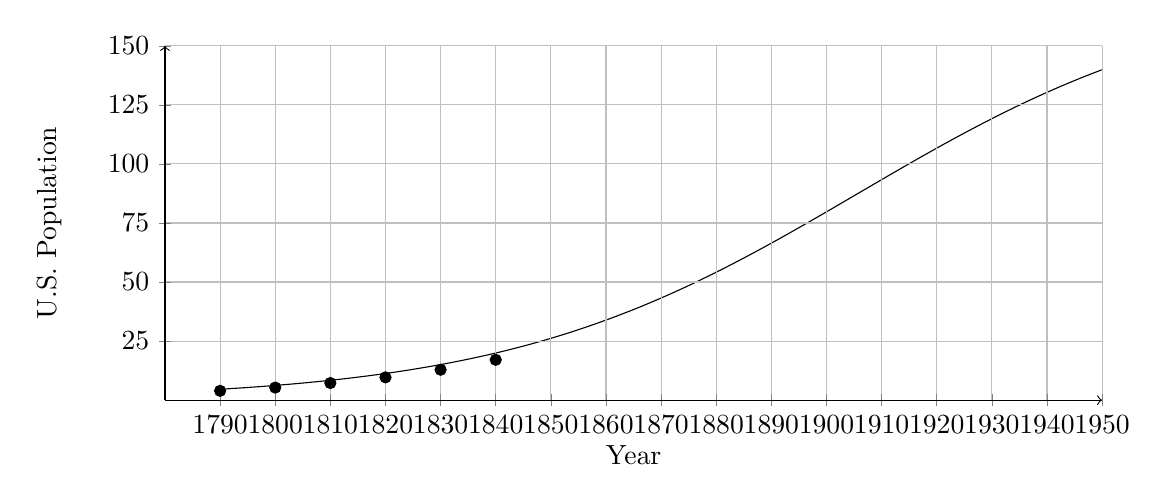
\begin{tikzpicture}
\begin{axis}[
    xmin=1780, xmax=1950,
    ymin=0, ymax=150,
    axis lines=center,
    axis on top=true,
    domain=0:1,
    x=0.07cm,
    y=0.03cm,
    xtick={1780,1790,...,1950},
    xticklabels={1780,1790,...,1950},
    ytick={0,25,...,200},
    yticklabels={0,25,...,200},
    axis lines=middle,
    axis line style={->},
    x label style={at={(axis description cs:0.5,-0.1)},anchor=north},
    y label style={at={(axis description cs:-0.1,.5)},rotate=90,anchor=south},
    xlabel={Year},
    ylabel={U.S. Population},
    grid=major
    ]
	\addplot[samples=100,domain=1790:1950] {175/(1+37.02*e^(-0.03121*(x-1790)))};
	\addplot [only marks] table {
	1790 3.929
	1800 5.308
	1810 7.24   
	1820 9.638
	1830 12.866
	1840 17.069
	};
\end{axis}
\end{tikzpicture}
\end{center}

The next graph shows the same model, but this time with data from the U.S. census filled in for the remaining years.
\begin{center}
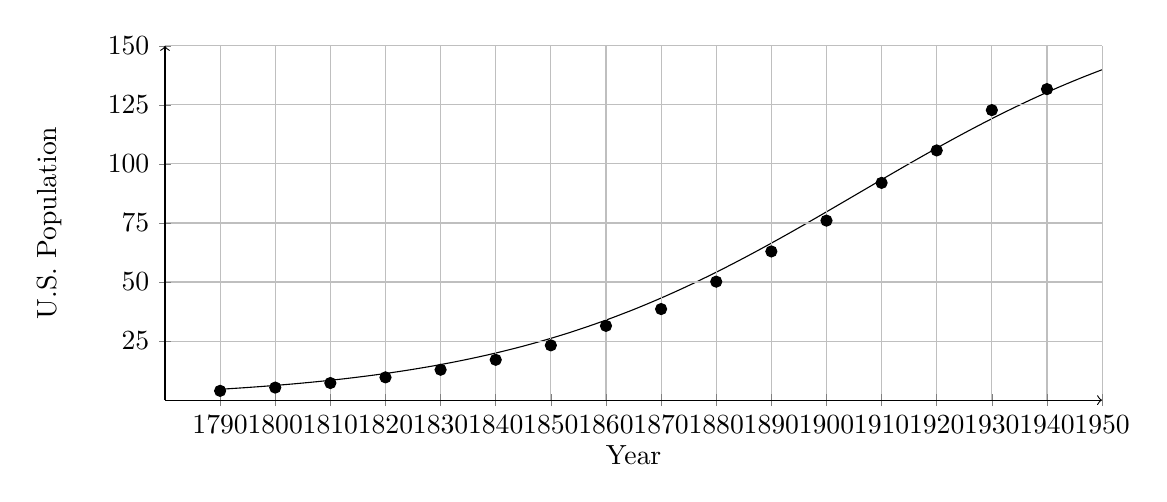
\begin{tikzpicture}
\begin{axis}[
    xmin=1780, xmax=1950,
    ymin=0, ymax=150,
    axis lines=center,
    axis on top=true,
    domain=0:1,
    x=0.07cm,
    y=0.03cm,
    xtick={1780,1790,...,1950},
    xticklabels={1780,1790,...,1950},
    ytick={0,25,...,200},
    yticklabels={0,25,...,200},
    axis lines=middle,
    axis line style={->},
    x label style={at={(axis description cs:0.5,-0.1)},anchor=north},
    y label style={at={(axis description cs:-0.1,.5)},rotate=90,anchor=south},
    xlabel={Year},
    ylabel={U.S. Population},
    grid=major
    ]
	\addplot[samples=100,domain=1790:1950] {175/(1+37.02*e^(-0.03121*(x-1790)))};
	\addplot [only marks] table {
	1790 3.929
	1800 5.308
	1810 7.24   
	1820 9.638
	1830 12.866
	1840 17.069
	1850 23.192
	1860 31.443
	1870 38.558
	1880 50.156
	1890 62.948
	1900 75.996
	1910 91.972
	1920 105.711
	1930 122.775
	1940 131.669
	};
\end{axis}
\end{tikzpicture}
\end{center}

Notice how closely the actual data tracks with the model's predictions; this is evidence of a good model, especially when we consider that the prediction was made ahead of time.  More often than you might expect, would-be experts will reach for data from the past and magically find a model that fits the data nearly perfectly, but such models tend to fail at making predictions, and they don't actually offer any insight.  A truly predictive model like this one with such accurate results is quite rare.
\pagebreak

\begin{example}[https://www.youtube.com/watch?v=mmL2H7_ynUA]{Rabbit Population}
A forest is currently home to a population of 200 rabbits.  The forest is estimated to be able to sustain a population of 2000 rabbits, and the rabbits can grow at a rate of 50\% per year.  Find a model to predict the future rabbit population, and draw a graph of this model.\\

\marginnote{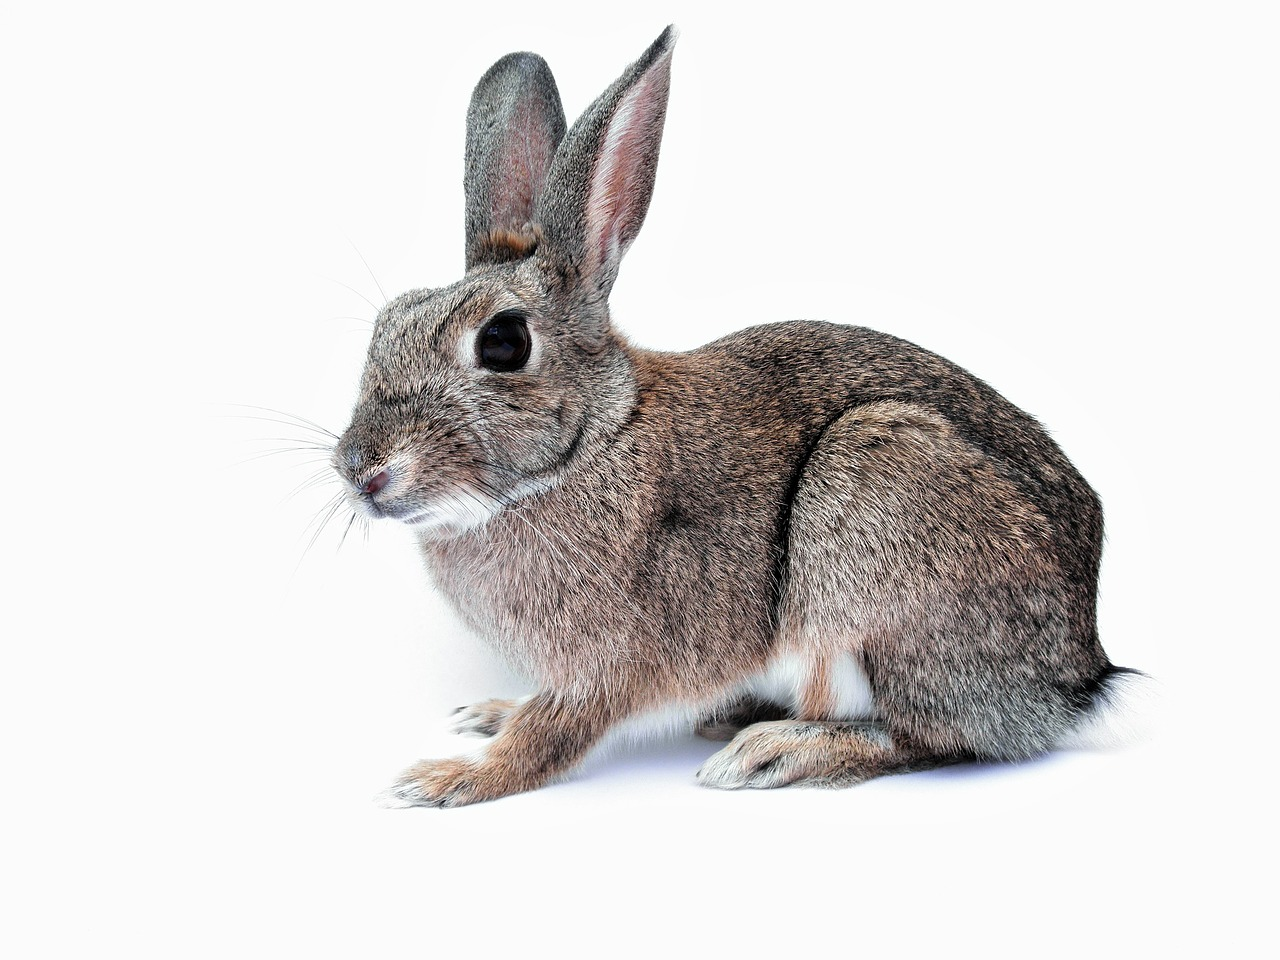
\includegraphics[scale=0.07]{Rabbit1}}
We're told that $r=0.5$, $M=2000$, and $P_0=200$.  Putting it all into the logistic model:
\begin{align*}
P_t &= \dfrac{M}{1+\left(\dfrac{M}{P_0}-1\right)e^{-rt}}\\
P_t &= \dfrac{2000}{1+9e^{-0.5t}}
\end{align*}

Graphing this equation:
\begin{center}
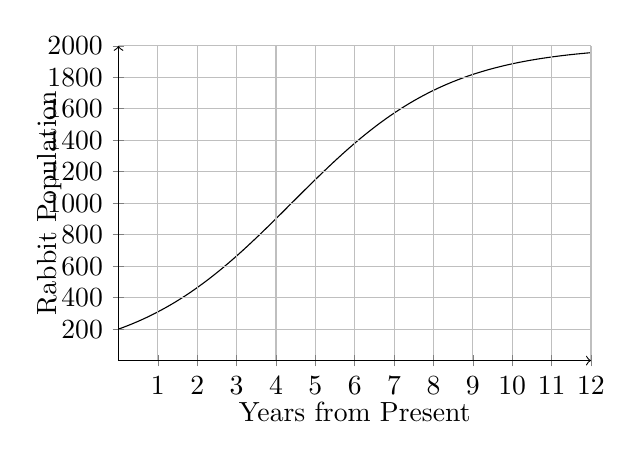
\begin{tikzpicture}
\begin{axis}[
    xmin=0, xmax=12,
    ymin=0, ymax=2000,
    axis lines=center,
    axis on top=true,
    domain=0:1,
    x=0.5cm,
    y=0.002cm,
    xtick={0,1,...,20},
    xticklabels={0,1,...,20},
    ytick={0,200,...,2000},
    yticklabels={0,200,...,2000},
    axis lines=middle,
    axis line style={->},
    x label style={at={(axis description cs:0.5,-0.1)},anchor=north},
    y label style={at={(axis description cs:-0.1,.5)},rotate=90,anchor=south},
    xlabel={Years from Present},
    ylabel={Rabbit Population},
    grid=major
    ]
	\addplot[samples=100,domain=0:12] {2000/(1+9*e^(-0.5*x))};
\end{axis}
\end{tikzpicture}
\end{center}

We can use this model to predict the rabbit population at any point in the future, and we note that according to the model, the rabbit population will level out near the carrying capacity in about 12 years.
\end{example}
\pagebreak

\begin{example}[https://www.youtube.com/watch?v=cd5xQCfLUZM]{Lizard Population}
On an island that can support a population of 1000 lizards, there is currently a population of 600.  These lizards have a lot of offspring and not many natural predators, so they have a very high growth rate of 150\%.  Use a logistic model to predict the lizard population 2 years from now.\\

\marginnote{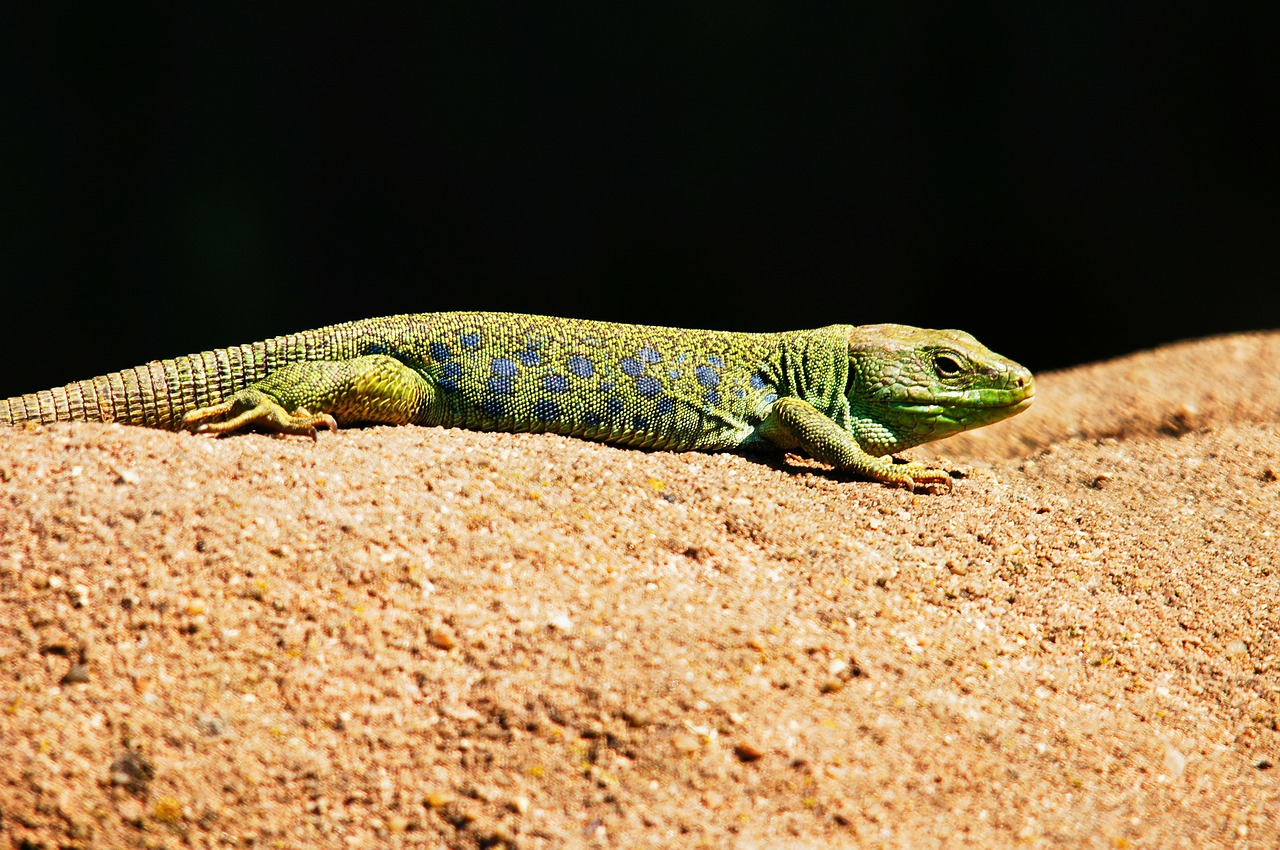
\includegraphics[scale=0.07]{Lizard1}}
Fill in the logistic model:
\begin{align*}
P_t &= \dfrac{M}{1+\left(\dfrac{M}{P_0}-1\right)e^{-rt}}\\
P_t &= \dfrac{1000}{1+\dfrac{2}{3}e^{-1.5t}}
\end{align*}

\begin{center}
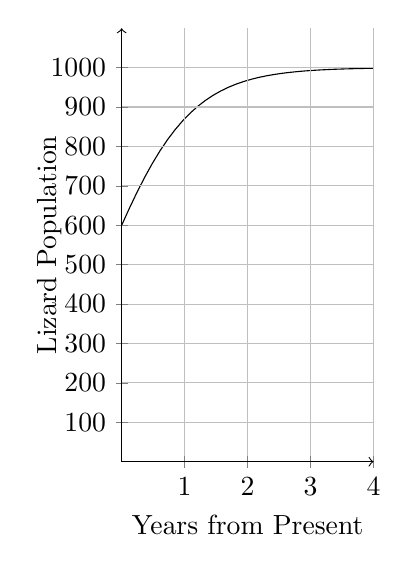
\begin{tikzpicture}
\begin{axis}[
    xmin=0, xmax=4,
    ymin=0, ymax=1100,
    axis lines=center,
    axis on top=true,
    domain=0:1,
    x=0.8cm,
    y=0.005cm,
    xtick={0,1,...,20},
    xticklabels={0,1,...,20},
    ytick={0,100,...,1000},
    yticklabels={0,100,...,1000},
    axis lines=middle,
    axis line style={->},
    x label style={at={(axis description cs:0.5,-0.1)},anchor=north},
    y label style={at={(axis description cs:-0.2,.5)},rotate=90,anchor=south},
    xlabel={Years from Present},
    ylabel={Lizard Population},
    grid=major
    ]
	\addplot[samples=100,domain=0:12] {1000/(1+(2/3)*e^(-1.5*x))};
\end{axis}
\end{tikzpicture}
\end{center}

Let $t=2$ to predict the population in 2 years:
\begin{align*}
P_2 &= \dfrac{1000}{1+\dfrac{2}{3}e^{-1.5(2)}}\\
 &= \dfrac{1000}{1+\dfrac{2}{3}\cdot 0.0498}\\
 &= \dfrac{1000}{1.0332}\\
 &\approx 968
\end{align*}
The model predicts that there will be approximately 968 lizards in 2 years.
\end{example}

\begin{try}[http://www.izzomath.com/103text/growthmodels/example3.1/story.html]
A field contains 20 mint plants, and the number of plants increases at a rate of 70\%, but the field can only support a maximum population of 300 plants.  Use the logistic model to predict what the population will be in three years.
\end{try}

\begin{exercises}

\ptwo{One hundred trout are seeded into a lake.  Absent constraint, their population will grow by 70\% a year.  If the lake can sustain a maximum of 2000 trout, use a logistic growth model to estimate the number of trout after 2 years.}
\ptwo{Ten blackberry plants started growing in a yard.  Absent constraint, blackberries will spread by 200\% a month.  If the yard can only sustain 50 plants, use a logistic growth model to estimate the number of plants after 3 months.}

\ptwo{A certain community consists of 1000 people, and one individual has a particularly contagious strain of influenza.  Assuming the community has not had vaccination shots and are all susceptible, the spread of the disease in the community is modeled by \[A = \dfrac{1000}{1+999e^{-0.3t}}\] where $A$ is the number of people who have contracted the flu after $t$ days.
\begin{enumerate}[(a)]
\item How many people have contracted the flu after 10 days?  Round your answer to the nearest whole number.
\item What is the carrying capacity for this model?  Does this make sense?
\item How many days will it take for 750 people to contract the flu?  Round your answer to the nearest whole number.
\end{enumerate}}
\ptwo{A herd of 20 white-tailed deer is introduced to a coastal island where there had been no deer before.  Their population is predicted to increase according to \[A = \dfrac{100}{1+4e^{-0.14t}}\] where $A$ is the number of deer expected in the herd after $t$ years.
\begin{enumerate}[(a)]
\item How many deer will be present after 2 years?  Round your answer to the nearest whole number.
\item What is the carrying capacity for this model?
\item How many years will it take for the herd to grow to 50 deer?  Round your answer to the nearest whole number.
\end{enumerate}}

\end{exercises}
